Please describe the basic characteristics of the software. 

Is is a web-based solution?

Ja

Is it installable or just available as a service? 

Die Software ist installierbar.



How much effort does the installation take (describe and give a time for the installation)?

Die folgenden Schritte werden auf folgendem Testrechner ausgef�hrt:

Ubuntu 12.04

Es wird die Free Trial Version von Nagios XI heruntergeladen unter:

http://www.nagios.com/products/nagiosxi

Die Trial Version ist eine 60 Tage Testversion von Nagios XI.

Es wird die VMware Virtual Machine (64-bit) Version 2012R1.6 heruntergeladen unter:

http://library.nagios.com/library/products/nagiosxi/downloads/main

Auf der viruellen Maschine l�uft CentOS 6.x und Nagios XI 2012 ist installiert.

Um die VMware Virtual Machine starten zu k�nnen, muss VMware installiert werden.
VMware kann kostenfrei heruntergeladen werden unter:

\url{https://my.vmware.com/web/vmware/free#desktop_end_user_computing/vmware_player/5_0}

Der heruntergeladene VMware-Player wird installiert mit:

sudo sh VMware-Player-5.0.1-894247.x86\_64.bundle

Der VMware-Player wird gestartet und es wird die virtuelle Maschine ausgew�hlt mit 

Open a virtual Maschine.

Die ausgew�hlte virtuelle Maschine wird gestartet mit 

play virtual maschine.

Die virtuelle Maschine wird gestartet. CentOS wird gebootet und Nagios gestartet.



Als n�chstes wird ein sicheres Kennwort vergeben. Damit kann auf Nagios XI �ber das Web Interface zugegriffen werden.

Dazu meldet man sich auf der virtuellen Maschine mit dem Root-Kennwort an.

Username: root

Password: nagiosxi

Als n�chstes wird mit 

passwd

ein neues Root Kennwort vergeben. Im folgenden wird es auf 111sonoma222 ge�ndert.

\begin{figure}[htp]
\centering
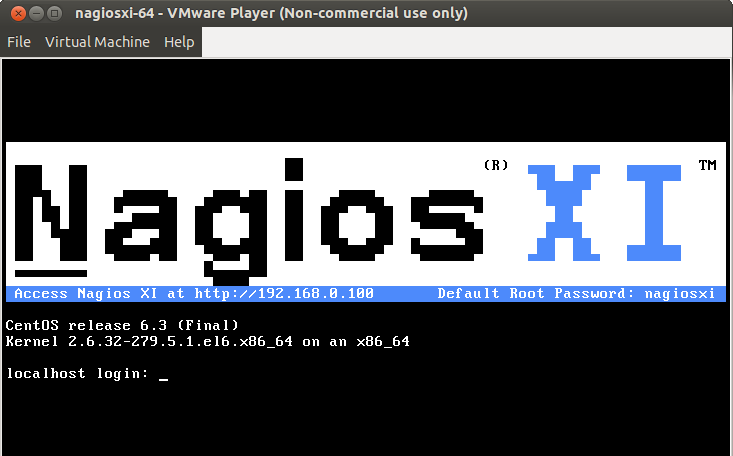
\includegraphics[width=0.6\textwidth]{ingo/bilder/virtuelleMaschine}
\caption{Nagios auf der virtuellen Maschine}
\label{fig:NagiosAufDerVirtuellenMaschine}
\end{figure}

Als n�chstes wird das MySQL Root Kennwort ge�ndert werden. Dazu wird der mysqladmin verwendet. Das Kennwort wird auf 111sonoma222 gesetzt

mysqladmin -u root -p'nagiosxi' password 111sonoma222

Als n�chstes sollte das MySQL Backup Script angepasst werden. Es wird im Backup Script das neue Kennwort 111sonoma222 angegeben.
Das Backup Script wird mit folgendem Befehl editiert.

nano /root/scripts/automysqlbackup

In diesem Script ist die Zeile 

PASSWORD=nagiosxi

zu �ndern in

PASSWORD=111sonoma222

Um die IP Adresse der virtuellen Maschine zu bekommen, wird folgender Befehl eingeben:

ifconfig

Hier steht unter eth0 $\rightarrow$ inet addr: 192.168.0.100

Mit dieser IP-Adresse kann auf des Web-Interface von Nagios XI zugegriffen werden.

In Abbildung \ref{fig:StartseiteVonNagios} auf Seite \pageref{fig:StartseiteVonNagios} ist die Starteseite von Nagios XI zu sehen.

\begin{figure}[htp]
\centering
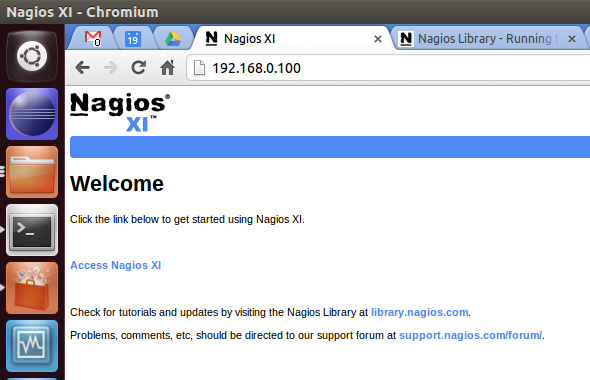
\includegraphics[width=0.6\textwidth]{ingo/bilder/Startseite}
\caption{Startseite von Nagios}
\label{fig:StartseiteVonNagios}
\end{figure}

Auf dem Web-Interface von Nagios kann auf Access Nagios XI geklickt werden, um Nagios XI einzustellen. Die Abbildung \ref{fig:NagiosXiEinstellen} auf Seite \pageref{fig:NagiosXiEinstellen} zeigt, dass an dieser Stelle folgende Punkte bearbeitet werden k�nnen:

\begin{itemize}
 \item die Prgramm URL, auf die die Nutzer auf Nagios zugreifen
 \item der Administratorname
 \item die EMail-Adresse des Administrators
 \item das Administrator-Kennwort
\end{itemize}

Nach einem Klick auf Install ist die Installation von Nagios XI fertig.

\begin{figure}[htp]
\centering
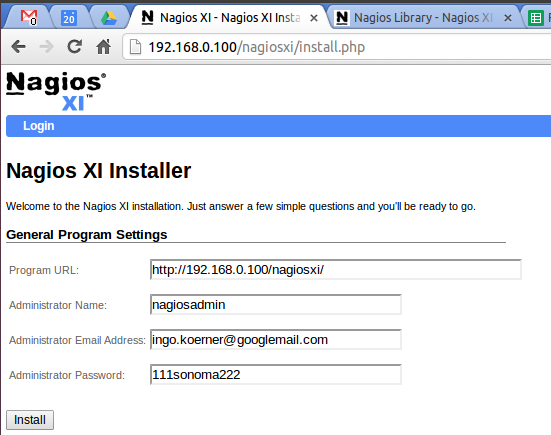
\includegraphics[width=0.6\textwidth]{ingo/bilder/NagiosInstall}
\caption{Nagios XI einstellen}
\label{fig:NagiosXiEinstellen}
\end{figure}

Leider kommt danach folgende Fehlermeldung, wie in Abbildung \ref{fig:NagiosXiFehlermeldung} auf Seite \pageref{fig:NagiosXiFehlermeldung} zu sehen. �ber das Web-Interface kann nicht mehr auf Nagios zugegriffen werden.

\begin{figure}[htp]
\centering
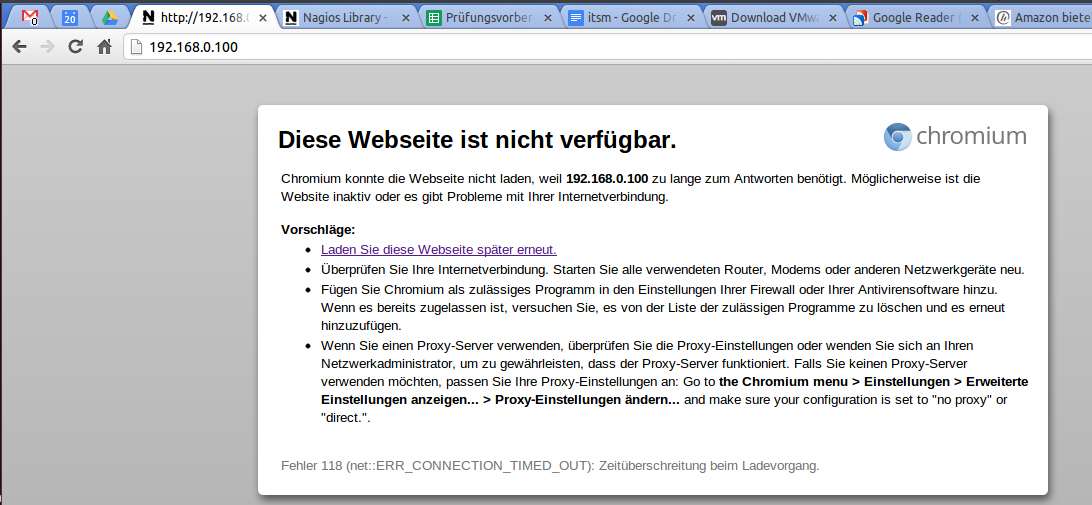
\includegraphics[width=0.6\textwidth]{ingo/bilder/NagiosFehler}
\caption{Nagios XI Fehlermeldung}
\label{fig:NagiosXiFehlermeldung}
\end{figure}



How old is the software? When did its development start? 

1999 ver�ffentlichte Ethan Galstad Nagios - dass damals noch NetSaint hie� - als Open Source Projekt.
http://www.nagios.org/about/history

Which version is it (0.1?)? 

Netsaint 0.0.1
\url{http://www.ussrback.com/UNIX/audit/netsaint/index.html}

Is it well established? How many customers are using it? 

Es wird gesch�tzt, dass es weltweit ca 1 Million Nagios Nutzer gibt.
http://www.nagios.org/about/community

Is it still further developed - are new releases planned and when was the last release?

Es wird immernoch weiterentwickelt. Neue Releases sind geplant. Die letzte Version 2012R1.6 ist von 15. Februar 2013.